\documentclass[10pt,10pt,10pt]{mugsthesis} % type size may be between 10-12 pt; default 12pt 

% load any additional packages you require
\usepackage{mathpazo}     % fonts; many alternatives here
\usepackage{lipsum}      % for blind sample text (testing only)
\usepackage{graphicx}    % for including graphics

% input macros (for example, write your own personal macros in a 
%   file called 'mymacros.tex' and uncomment the next line)
%\include{mymacros}

% place your title here, using `\\' to break the lines 
% of the title into the requested inverted pyramid layout
% the title must not exceed 120 characters
\title{ % thesis title in inverted pyramid layout
  A STUDY OF THE SOCIOLOGICAL IMPACT OF THE\\
  1984 OLYMPICS ON THE POVERTY\\
  LEVEL OF CITIZENS OF\\
  LOS ANGELES
} % note: \\ are line breaks in the title

\author{John J. Smith, B.A.} % your name and credentials
\degree{Master of Science}   % the degree
\degreemo{December}          % the degree month (always May, August, or December)
\degreeyr{2013}              % the degree year

% set the smallest sectional units that are numbered and appear in the contents
%\maxsecnumdepth{subsubsection} % default: subsection
%\settocdepth{subsubsection}    % default: subsection

% end the preamble and begin the document
\begin{document}

\maketitle                % create a title page from the preamble info

\frontmatter
This document gives a quick, relatively minimal example of the use of
\texttt{uafthesis.cls}, while trying to show its features.

This section is contained in \texttt{abstract.tex}.
        % include the abstract.tex file; not to exceed 350 words
%%% Acknowledgements
%%% ----------------------------------------------------------------------
\begingroup
% you can erase the following three lines if you do not use an introductory quote
\cleardoublepage
\let\clearpage\relax
\let\cleardoublepage\relax
\begin{flushright}\slshape
	Put your fancy quote here. Or don't. \\ \medskip
	--- Awesome Author
\end{flushright}

\bigskip
\otherlanguage{ngerman}

\addchap{Vorwort}

\blindmathfalse
\blindtext

\bigskip

\begin{flushright}
	Place, \doctime
\end{flushright}

\endgroup % include an acknowledgments.tex file, OPTIONAL
%% File containing the dedication
%% Do not write anything between the curly braces of the \chapter*
%% command unless you want the dedication to show up in the table
%% of contents.

\chapter*{}

\begin{HECdedication}
%% Writte your dedication here.
\end{HECdedication}
      % include a dedication.tex file, OPTIONAL

\tableofcontents          % generate and include a table of contents
\listoftables             % use this if you have tables
\listoffigures            % use this if you have figures (AFTER LoT if you have both)

\mainmatter
% include .tex files containing the text of each individual chapter
\chapter{Introduction} \label{cha:intro}
Here is some introductory text regarding the thesis.
Ideally, the introduction should be longer than one page. 
This way, the reader will have some vague idea of what it is that you'll be presenting.

I have added liberal blind text here to extend this chapter onto a second page.  
We can then check the pagination and other important things. 
This chapter should be introducing the topic of your thesis and providing motivation to your work.

Figure~\ref{fig:test2} shows a sample figure. More details are discussed in Appendix~\ref{app:test}.
\begin{figure}
  \centering 
  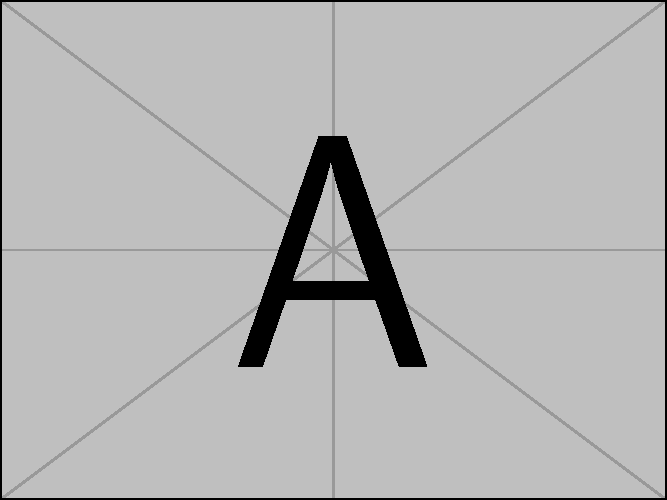
\includegraphics[width=1in]{example-image-a}
  \caption{This test figure tests captions and Table of Contents 
    behavior for very lengthy captions.}
  \label{fig:test2}
\end{figure}

\section{Background}
Test sectioning commands.  We can also have \verb+subsection+, \verb+subsubsection+,
\verb+paragraph+, and \verb+subparagraph+.  Let's try a few:

\subsection{Test Subsection}
\lipsum[1]

\subsection{Another Subsection}
Testing display mathematics:
\begin{equation}
e = mc^2,
\end{equation}
where $e$ is the energy, $m$ is the mass, and the constant $c$ represents the speed of light in a vacuum.

\subsubsection{Subheading}
\lipsum[3-5]

\chapter{Literature Review} \label{cha:litreview}
As you can see here, the author has performed an exhaustive literature review to provide
a solid foundation on which the remainder of this thesis is built.
\begin{quote}
This is a test of the \verb+quote+ environment. We should be in single-spaced mode and with some additional indentation to set this off from the rest of the text.
\end{quote}
Now we should have returned to double-spaced mode and regular indentation/margins.
Let's add some more text here to fill the page and check the glue settings.
We need more text on this page for testing purposes.

Now let's test the \verb+quotation+ environment:
\begin{quotation}
This is a test of the \verb+quotation+ environment. We should be in single-spaced mode and with some additional indentation to set this off from the rest of the text.
\end{quotation}
Here we return%
\footnote{
  This is a test footnote extending over more than one line. 
  This should be in single-spaced mode according to the MUGS Thesis Directives.
} 
to normal text mode.

\lipsum
\nocite{*} % dump all references for testing purposes

% uncomment next line to change bibliography name to references (depends on style guide used)
%\renewcommand{\bibname}{REFERENCES}
\bibliography{refs}       % use a bibtex bibliography file refs.bib
\bibliographystyle{plain} % use the plain bibliography style (many options here)

% switch to appendix chapter numbering and include appendices
\appendix
\chapter{Test Appendix with a very long title in order to test spacing behavior} \label{app:test}
\lipsum[2]

A convenient form for representing substantial numerical or textual data is a table. 
Table~\ref{tab:test} shows an example of this functionality in \LaTeX.
\begin{table}
  \centering
  \caption{Test table. With an extra-long caption to test spacing functionality for table captions. And inline mathematics.}
  \begin{tabular}{lrr}
    \toprule
    Heading 1 ($u_x$)  & Head 2 & Head 3 \\
    \midrule
    Analytical         & 1.000  & 1.000  \\
    Forward Difference & 0.973  & 0.976  \\
    \bottomrule
  \end{tabular}
  \label{tab:test}
\end{table}
Diagrams, plots, and other graphics should be placed in figures. 
Figure~\ref{fig:test} shows an example of such an environment.
The command \verb+\includegraphics+ from the \verb+graphicx+ package may be used to include external graphics in a wide variety of formats.
\begin{figure}
  \centering 
  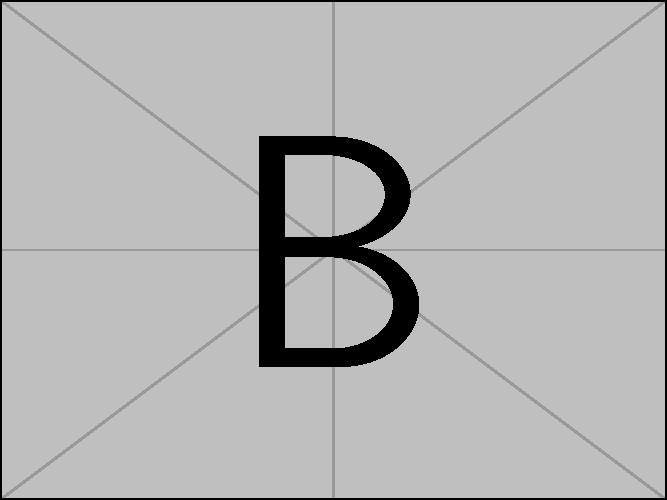
\includegraphics[width=1in]{example-image-b}
  \caption{This test figure tests captions and Table of Contents 
    behavior for lengthy captions.}
  \label{fig:test}
\end{figure}

\section{This is a Very Long Heading to Test the Table of Contents Behavior for Very Long Section Headings}
Sample text. Sample text.

\subsection{This is an Extremely Long Subsection Heading to Test Spacing Behavior for Subsections}
\lipsum[3]

\subsubsection{This is an Extremely Long Subsubsection Heading to Test Spacing Behavior for Subsubsections}
\lipsum[4-5]


\end{document}

